\section{Introduction}

The main contribution to this dissertation is the automatic construction of a database of experimental data.
We created SuperCon\textsuperscript{2} by processing 37770 research articles and obtaining 40324 records of superconductors materials with their respective properties and conditions, including \tc, applied pressure measurement methods. 
We applied traditional methods such as Machine Learning to a new field, using a novel data flow that ingests PDF documents (Chatpter~\ref{cha:pdf_extraction}), extracts materials and properties (Chapters~\ref{cha:extraction-experimental-data} and~\ref{cha:measurements}) and deliver an aggregated dataset. 
Our work created a novel TDM flow approach for material informatics. We processed a batch of PDF articles belonging to the category \textit{ cond-mat.supr-cond} in ArXiv. Compared with other methods, our work does not need to be adapted to the data source, whether it is ArXiv, BioRXiv, ChemRXiv, or any proprietary publisher article.  
Compared to the original SuperCon, SuperCon\textsuperscript{2} was collected in a few days and counted 2052 triplets with applied pressure (\textit{material-\tc-pressure}), and 3602 records with an explicit measurement method (\textit{material-\tc-measurement method}).
However, given the strict quality requirements that SuperCon must meet, the data must be validated by humans and therefore SuperCon\textsuperscript{2} is not a replacement for SuperCon. 
In this chapter, we discuss how SuperCon\textsuperscript{2} is built, including the technical information about the data format and the processing. 
In chapter~\ref{cha:curation} we address data quality by discussing our solution to guarantee high data quality with an optimised process. 


\section{Database construction}
\label{sec:ingestion}

The ingestion process (Figure~\ref{fig:map-reduce}) is designed using an Extract-Aggregate approach, implemented through grobid-superconductors (see chapters~\ref{cha:pdf_extraction} and~\ref{cha:extraction-experimental-data}).

\begin{figure}[htbp]
  \centering
  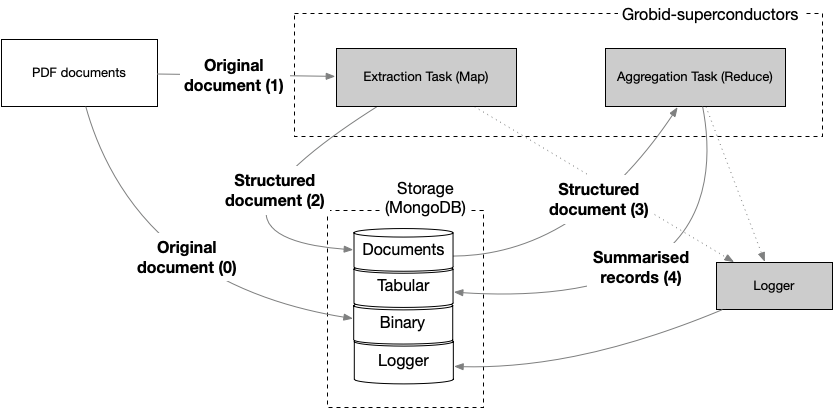
\includegraphics[width=\textwidth]{figures/curation/ingestion-schema.png} 
  \caption{Ingestion process}
  \label{fig:map-reduce}
\end{figure}

Storage is implemented using MongoDB~\footnote{\url{https://www.mongodb.com}}, an open source document database, and the collections are designed as different stages in the processing: 
\begin{itemize}
    \item the \textbf{binary} collection contains the original PDF documents 
    \item the \textbf{documents} collection contains the structured document
    \item \textbf{tabular} collection stores the summarised records, and finally 
    \item \textbf{logger} contains detailed information on the status of the process of each document, including eventual errors information. More details are given in Section~\ref{subsec:curation-and-processing-logs}.
    \item \textbf{training\_data} Used to collect training examples in and discussed in Section~\ref{subsec:feedback-loop-training-data}.
\end{itemize}


The "Extraction Task" takes the PDF documents in input and transforms them into a rich representation document that includes text passages (sentences, paragraphs), annotations, and tokens as JSON files, which we will refer to as \textit{structured documents} (Figure~\ref{fig:data-flow-2}). 

\begin{figure}[htbp]
  \centering
  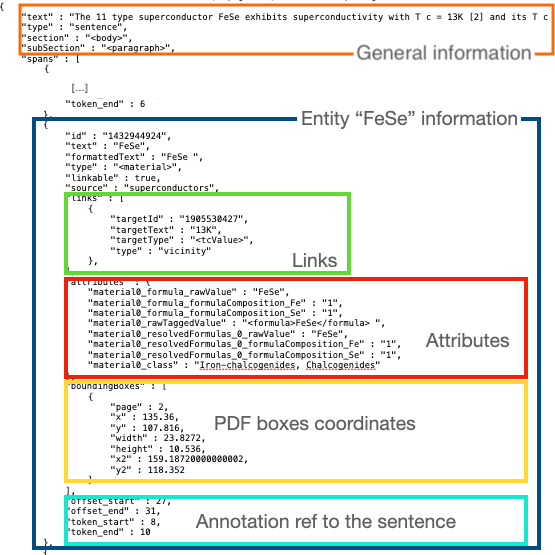
\includegraphics[width=0.8\textwidth]{figures/curation/data-flow-2} 
  \caption{Example of the information from one single entity from a passage extracted in the "Extraction Task". The different structured information are highlighted: links, attributes, PDF boxes coordinates (to visualise annotations on the PDF document), and annotations references within the passage (to visualise annotations on text).}
  \label{fig:data-flow-2}
\end{figure}

Each passage is composed of the following attributes: the text of the passage, the type (whether it is a sentence or paragraph), the main section: header, body, and annex, and the subsections: title, abstract, paragraph, caption.
Furthermore, a passage also contains the list of spans representing the extracted entities and a list of layout tokens. 
The spans are characterised by text, type, attributes, a unique identifier, and other internal information (e.g. from which ML model the entity was extracted). 
The attributes are stored as a key-value and mainly contain information extracted by the material parser such as, for example, the chemical formula, the structured composition, the material class, and so on.
The layout tokens contain low-level information coming from the PDF document: font size, font face, superscript, subscript, bold, italic, and coordinates within the PDF document. The coordinates are a couple of x,y numbers that are used to build annotation "boxes" to encapsulate each token independently (see Figure~\ref{fig:pdf-view} in the following chapter, as an example). 

The "Aggregation Task" takes the structured document as input and reduces it to a table format where each row (referred to as a \textit{summarised record}, or, simply \textit{record}) pivots around the relation materials-Tc and attaches additional elements to it. 
The number of aggregated records can increase when large entities are extracted and may contain condensed information referring to multiple materials. 
For example, the raw material "Zn and CU doping La Fe B" will be aggregated as two records (doping: Zn, formula: La Fe B) and (doping: Cu, formula: La Fe B). 

In the following listing, we illustrate an example of aggregated record: lines 2-21 contain the records information such as material name, \tc, pressure, etc. Lines 22-34 represent the list of spans, which are the original annotation information. They are used to link the aggregated records back to the original structure document information. 
Line 35, 'hash' is a unique signature of the original document using the first 10 characters of the MD5 hash function on the binary content. We use this information to link the original document, the structured document, and the summarised records.
'type', 'timestamp' and 'status' are internal workflow information, discussed in the next chapter. 
The rest of the lines contains the bibliographic data (39-42).

\begin{lstlisting}[numbers=left,numbersep=5pt,caption=Example of record related to the FeSe material after the aggregation.]
{
  "_id": ObjectId("63dcae91e4d716dd10dd5a7d"),
  "rawMaterial": "FeSe",
  "materialId": "1432944924",
  "name": null,
  "formula": "FeSe",
  "doping": null,
  "shape": null,
  "materialClass": "Chalcogenides, Iron-chalcogenides",
  "fabrication": null,
  "substrate": null,
  "variables": null,
  "criticalTemperature": "13K",
  "criticalTemperatureId": "1905530427",
  "measurementMethod": "",
  "measurementMethodId": "",
  "appliedPressure": null,
  "appliedPressureId": null,
  "section": "body",
  "subsection": "paragraph",
  "sentence": "The 11 type superconductor FeSe exhibits superconductivity with T c = 13K [2] and its T c reaches 37K under high pressure (4-6 GPa) [3,4].",
  "spans": [
    {
      "id": "1432944924",
      "text": "FeSe",
      "type": "<material>",
      "linkable": false,
      "offset_start": 27,
      "offset_end": 31,
      "token_start": 0,
      "token_end": 0
    },
    [...]
  ],
  "hash": "f70a71214f",
  "type": "automatic",
  "timestamp": ISODate("2022-11-24T09:02:53.256Z"),
  "status": "new",
  "title": "Evidence of Inhomogeneous Superconductivity in FeTe1-xSexby Scotch-Tape Method",
  "doi": "10.1143/jpsj.81.113707",
  "authors": "Hiroyuki Okazaki, Tohru Watanabe, Takahide Yamaguchi, Yasuna Kawasaki, Keita Deguchi, Satoshi Demura, Toshinori Ozaki, Saleem. J. Denholme, Yoshikazu Mizuguchi, Hiroyuki Takeya, Yoshihiko Takano",
  "publisher": "Physical Society of Japan",
  "journal": "Journal of the Physical Society of Japan",
  "year": 2012
}
\end{lstlisting}





\section{Results}
\label{sec:results-supercon2}

SuperCon\textsuperscript{2} represents the result of our effort to build an automatic TDM process to automatically extract experimental data. 

Compared to the original SuperCon, SuperCon\textsuperscript{2} was collected in a few days. There is no information about how SuperCon was constructed, only that it started in 1987~\cite{ishii2023structuring}. 
When we built the new process to obtain SuperCon\textsuperscript{2}, we were asked to consider two information: ``applied pressure'' and ``measurement method''. 
``Applied pressure'' is the pressure applied to make the material a superconductor and has gained attention because it can radically change the physical structure of a material. Still, at the time of writing, there have been studies that consider this property for material informatics. 
On the other hand, ``measurement method'' is the way scientists measured the superconducting transition temperature \tc and can be used to semantically recognise multiple \tc obtained from the same material or sample. In particular, the identification of calculated properties is fundamental when providing data for predictions. 
These properties were present only for a minority of records in SuperCon and, we hypothesise, that they were not considered in the initial design. The fact that applied pressure was recorded in different fields of the database suggests that such action was more a decision of the curator than a methodological change.
The resulting SuperCon\textsuperscript{2} counted 2052 triplets with applied pressure (\textit{material-\tc-pressure}), and 3602 records with an explicit measurement method (\textit{material-\tc-measurement method}).
The SuperCon\textsuperscript{2} schema is discussed in~\ref{sec:results-supercon2} with examples in Table~\ref{tab:supercon2-schema}. 

However, our TDM process is limited to text, whereas the manual process has also been focussing on plots and tables. This limitation reduces the density of the data that is collected, as observed by the amount of information (33,000 records) extracted from only 7227 articles. Such additions should be built as separate projects.
However, the automatic process cannot be used without manual validation given the high-quality constraints of SuperCon. This gives the opportunity to combine the TDM process with data curation in a homogeneous flow that is described in Chapter~\ref{cha:curation}.

\begin{table}[htpb]
    \centering\small
    \begin{tabular}{lcc}
        \toprule
        \textbf{Category} & \textbf{SuperCon} & \textbf{SuperCon\textsuperscript{2}} \\
        \midrule
        Size (records) & $\sim$33000 & 40324 \\
        Size (papers) & 7227 & 37700 \\
        \# records with applied pressure & 6 & 2052 \\
        \# records with measurement method & 600 & 3602 \\
        Process & Manual & Automatic \\
        Time for process & N/A & A few days \\
        Scope & Text, plots, tables & Text \\
        \bottomrule
    \end{tabular}
    \caption{Comparison in volumes from Supercon and SuperCon\textsuperscript{2}.}
    \label{tab:comparisong-supercon-supercon2}
\end{table}



\afterpage {
    \clearpage % Flush earlier floats (otherwise order might not be correct)
    
    \begin{table}[ht]
        \centering\small
        \caption{Summary and description of the SuperCon\textsuperscript{2} schema. ``Internal information'' is technical information not accessible to the users.}
        \scalebox{0.8}{
            \begin{tblr}{Q[l,m]Q[r,m]Q[r,m]}
                \hline[1pt]
                \textbf{Field name} & \textbf{Description}                             & \textbf{Examples}             \\
                \hline
                \SetCell[c=3]{c}{\emph{Material information}}                                                        \\
                \hline[dashed]
                {Raw                                                                                                   \\ material} & The material or sample as it appears in the text &\\
                \hline[dotted]
                Name                & Canonical name of a material                     & {PCCO, PCO, Metal diboride,   \\ hydrogen, carbon} \\
                \hline[dotted]
                Formula             & {Material expressed as chemical formula. This                                    \\ includes also formulas with stochiometric variables} & {$Pr_{1.869}Ce_{0.131}CuO_4-\delta$,\\ $MgB_2$, $La_{2-x} Sr_x CuO_4$} \\
                \hline[dotted]
                Doping              & {Doping ratio and doping materials                                               \\ that might be adjoined to the material} & {Overdoped, underdopded,\\ optimally doped,\\ bulk, pure, 1\% Zn, Zn\\ (from Zn-doped XYZ)}\\
                \hline[dotted]
                Shape               & The shape of the material or the sample          & {Single crystal, polycrystal, \\ wire, powder, film} \\
                \hline[dotted]
                Variables           & Variables that can be substituted in the formula & x = 0, RE=Ln,St               \\
                \hline[dotted]
                Class               & {Material classification according                                               \\ to the domain-experts taxonomy} & cuprates, oxides, and alloys\\
                \hline[dotted]
                Fabrication         & {All the information that does not                                               \\ belong to any of the previous tags} &  {Intercalated,\\ synthesized by MBE method,\\ electron-doped, hole-doped} \\
                \hline[dotted]
                Substrate           & Substrate material described in the raw material & {PCCO films onto              \\ $Pr_2 CuO_4 (PCO)/SrTiO_3$ }\\
                \hline[dashed]
                \SetCell[c=3]{c}{\emph{Properties}}                                                                  \\
                \hline[dashed]
                {Critical                                                                                              \\ Temperature}  & Superconducting critical temperature &\\
                \hline[dotted]
                {Applied                                                                                               \\ Pressure}  & {Pressure applied when measuring \\ the superconducting critical temperature} &\\
                \hline[dotted]
                {Measurement                                                                                           \\ Method}  & {Method for measurement of the\\ superconducting critical temperature} & {Magnetic susceptibility,\\ specific heat, calculation,\\ prediction, resistivity}\\
                \hline[dashed]
                \SetCell[c=3]{c}{\emph{Document bibliographic information}}                                          \\
                \hline[dashed]
                Section             & The main body section of the paper               & Header, body, annex           \\
                \hline[dotted]
                Subsection          & The secondary segmentation area of the paper     & {Paragraph, table caption,    \\ figure caption, title, abstract} \\
                \hline[dotted]
                {Authors,                                                                                              \\ Title, DOI,\\ Publisher,\\ Journal, Year} & \SetCell[c=2]{c}{Bibliographic information of the document}\\
                \hline[dashed]
                \SetCell[c=3]{c}{\emph{Internal information}}                                                        \\
                \hline[dashed]
                {Hash,                                                                                                 \\ Timestamp} & \SetCell[c=2]{c}{Hash calculated on the binary content of the original PDF\\ document and the timestamp when the document was processed.}\\
                \hline[1pt]
            \end{tblr}
        }
        
        \label{tab:supercon2-schema}
    \end{table}
    \clearpage
}




\section{Conclusions}

This contribution represents the main contribution of this dissertation where our efforts are applied in collecting SuperCon\textsuperscript{2}, which is a database with 40324 records of superconductors materials and properties, including the applied pressure and the \tc~measurement method.
SuperCon\textsuperscript{2}. 
This database is available in various formats at \url{https://github.com/lfoppiano/supercon}.

SuperCon\textsuperscript{2} should not be considered as a replacement of SuperCon but as a staging are where automatically extracted data is collected. Domain-experts can access this data, correct it and push it to SuperCon. 
This approach will reduce the amoutn of human labor required and improve the overall quality of the data, as we demosntrate in the next Chapter~\ref{cha:curation}.